%  <-- ezzel lesznek jelölve a kommentek,
%a legtöbb dolgot jobb békénhagyni úgy ahogy van, általában csak {} közé vagy \section{} alá kell írni majd
%az ITKproc miatt nem kell megformáznod a szöveget tehát ezt mindenképpen hagyjátok a itt, valamint mindig legyen a dokumentum mappájában, hogy elérje a fordító
\documentclass[10pt, conference,a4paper]{ITKproc}

\usepackage[utf8]{inputenc}
\usepackage{graphicx}
\usepackage{gensymb}
\graphicspath{ {images/} }
% correct bad hyphenation here

\hyphenation{pre-sence vi-su-alized si-mu-la-tions mo-le-cu-lar se-ve-ral cha-rac-te-ris-tic CoNSEnsX}


\begin{document}
% ide a {} közé írd a jegyzőkönyv címét
\title{GPS mérési jegyzőkönyv}
% ezek gondolom egyértelműek, itt is mindig csak a {} szerkesszétek, valamint használhattok \\ sortöréshez, pl dátum hozzáírás stb
\author{\IEEEauthorblockN{Mátyás Antal}
\IEEEauthorblockA{(Supervisor: Attila Tihanyi)\\
Pázmány Péter Catholic University, Faculty of Information Technology and Bionics\\
50/a Pr\'ater street, 1083 Budapest, Hungary\\
\texttt{antal.matyas.gergely@hallgato.ppke.hu}}
}


\maketitle

\begin{abstract}
A mérés célja volt a mikrokontrollerek gyakorlati megismerése, az MSP 430-196 mikrokontroller használata, egyszerű alapműveletek végrehajtása, ezzel a flag bitek működésének gyakorlati vizsgálata. 
\end{abstract}

\IEEEpeerreviewmaketitle
% innentől kezdve jönnek a feladatok
% \section{} Ezzel hozunk létre fejezetet, a {} közé pedig bármi írhatunk, általában úgyis "Feladat" és "összefoglalás"-t fogunk,
% a fejezetek alapjáraton számozódnak római számokkal tehát azt nem szükséges beleírni, 
% ha alfejezeteket akarunk létrehozni akkor \subsection{} subsubsection{} stb- vel tegyük
%példa:
\section{Mérendő objektumok}

A mérés során az MSP 430-196 mikrokontrollert, valamint egy számítógépet és az ezen futó programozási környezetet használtunk, ennek segítségével végeztünk a mikrokontrolleren egyszerű alapműveleteket, összeadást és kivonást, ezzel ismerkedve a műveletvégzéssel, valamint a flagek használatával. A mérés során a műveletek elvégzésére használt programrészleteket a jegyzőkönyvbe illesztem, valamint az elkészült programot az emailhez csatolom. 

\section{8 bites összadás}
\subsection{Előjel nélkül}
Két szám összeadásához a $mov.b$ parancs használatával az R4-es és R5-ös regiszterbe töltöm, majd az $add.b$ parancs segítségével összeadom őket. Ennek eredményeképp az R4-es regiszterbe kerül a művelet eredménye. A parancsokban a $.b$ jelző a byte-ra utal, ennek segítségével végzünk műveleteket 8bites környezetben. \\
Kipróbáltam továbbá a következő műveletet, mely a 8bites környezetben való műveletvégzésnél megjelenő túlcsordulásra példa. Mivel 8biten tárolható legnagyobb érték a $2^8 - 1 = 255$, a példában ehhez a számhoz adtunk hozzá 1-et. A kapott érték a túlcsordulás miatt 0 lesz, megfigyelhető azonban a carry bit 1-es értéke. 
\subsection{Előjellel}
Túlcsordulás nélkül az előjeles környezetben való műveletvégzés azonos módon történt, mint előjel nélkül. Túlcsordulást tesztelve azonban összeadtam a 127 és 1 számokat - az előjel miatt a tárolható számok maximális értéke a felére csökkent - az eredménynél az overflow bit 1-es értékre változott. 

\begin{figure}[h]
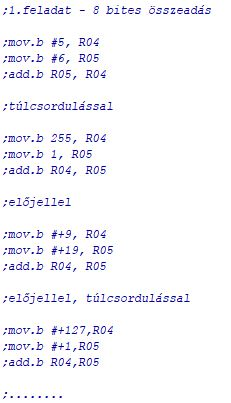
\includegraphics[scale=0.5]{1feladat}
\centering

\end{figure}

\section{16 bites összeadás}
\subsection{Előjel nélkül}
Az összeadás a 8biteshez hasonlóan működik. Itt azonban a $mov.w$ paranccsal töltjük az 5 és 6 számokat az R4 és R5 regiszterekbe, majd az $add.w$ paranccsal adjuk őket össze, ezzel az eredményt az R4 regiszterhez rendelve. A $.w$ itt a word rövidítése, mivel 16bites környezetben dolgozunk. 
\\
Túlcsordulásra itt a 65535 valamint 3 számot adtuk össze, hiszen a maximális tárolható számérték a $2^16 - 1 = 65535$. Az előző feladathoz hasonlóan a túlcsordulás miatt itt is 1-es carry bit értéket kapunk. 
\subsection{Előjellel}
A 8bites környezethez hasonlóan, előjeles környezetben itt is csökken a tárolható érték, hiszen 15bit tárolja a számértéket, az első pedig az előjelet jelzi, így a maximális érték $2^15 - 1 =32767$. A műveletvégzés után megfigyelhető, hogy az eredmény negatívvá válik, valamint az overflow és negatív bit értéke 0 lesz. 

\begin{figure}[h]
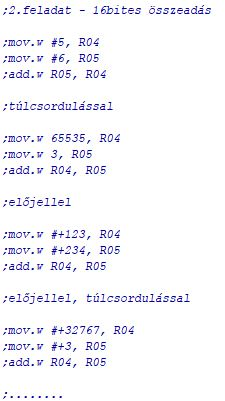
\includegraphics[scale=0.5]{2feladat}
\centering

\end{figure}

\section{32 bites összeadás}
\subsection{Előjel nélkül}
A mikrokontroller regiszerei csak 16bites értékek tárolására alkalmasak, így a 32bites műveletek elvégzéséhez minden szám tárolására két datab regisztert használtunk. Egyikben tároltuk a szám nagyobb helyiértékű tagját, a másodikban pedig a kisebbet. A műveletvégzés során először összeadjuk a kisebb helyiértékű tagokat, majd a carry bit figyelembevételével a nagyobb értékeket is, ezt az $addc.w$ parancs segítségével. 
\subsection{Előjellel}
Az előjeles összeadás egyben példa a túlcsordulásra is. Az alacsonyabb helyiértékű tagot előjel nélkül, a magasabbat viszont előjeles ábrázolásban használjuk. A képen található kód javítva lett, az utolsó művelet itt is $addc.w$. 

\begin{figure}[h]
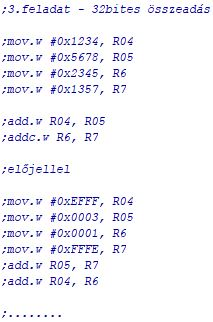
\includegraphics[scale=0.5]{3feladat}
\centering

\end{figure}

\section{8 bites kivonás}
\subsection{Előjel nélkül}
A kivonás előjel nélküli számok esetén az összeadáshoz hasonlóan történik. A $sub.b$ parancs használatával hajtottuk végre a műveletet. Amennyiben az intervallumból kilépünk, tehát az eredmény negatív lenne, a számkezelés újraindul a maximumtól. A fenti példában az R4 regiszterből vonjuk ki az R5öst, az eredmény negatív, így a regiszter értékében tapasztaltuk a fent említett jelenséget. 
\subsection{Előjellel}
Az előjeleket a szám elé írva jelezzük az értéküket. Az overflow bit értéke 0, tehát az eredmény előjele megfelelő. 

\begin{figure}[h]
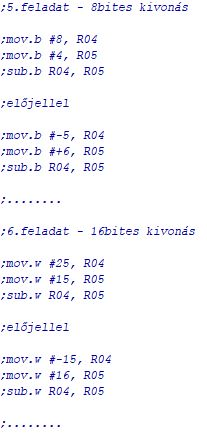
\includegraphics[scale=0.5]{56feladat}
\centering

\end{figure}

\section{16 bites kivonás}
\subsection{Előjel nélkül}
A kivonás az előzőekhez hasonlóan működött, a $sub.b$ parancsot azonban a $sub.w$-re cseréltük. Amennyiben a 25ből vontuk ki a 15öt, a művelet elvégezhető volt, viszont ha fordított sorrendben, a számozás újraindult. 
\subsection{Előjellel}
Előjeles környezetben a művelet a 8bitessel azonos módon működött. 
\section{32 bites kivonás}
\subsection{Előjel nélkül}
Az eddigiekhez hasonlóan a számokat két regiszterben tároltuk, a magasabb helyiértékűek kivonásánál a $subc.w$ parancs segítségével a borrow bit értékét is figyelembe vettük. Az eredmény az elvárt $2^32 - 1 - 1 = 4,294,967,294$ értéket vette fel. 
\subsection{Előjellel}
Előjeles környezetben a kivonás hasonló módon történt. 

\begin{figure}[h]
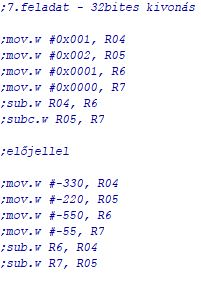
\includegraphics[scale=0.5]{7feladat}
\centering

\end{figure}

%Ha szeretnéd hogy az adott fejezet ne legyen számozva használj \section*{} -t, pl Acknowledgements


% Az egyenletekre, táblázatokra, listákra stb. itt nem térnék ki, ahhoz mindenképp érdemes kicsit utána olvasni

% A references mindig a legutolsó fejezet lesz

%  minden hivatkozás elnevezünk, ezzel a névvel fogunk hivatkozni a szövegen belül
% \bibitem{} <- hivatkozásnév
% A hivatkozás formája legjobban a példa dokumentumban látszik a tanárúr honlapján, általában: szerző, olvasott anyag neve, közreműködők, hely, év
% a szövegben pedig \cite{Megadott hivatkozásnév} -vel hivatkozunk


% példa:


% Ez a rész mindig marad:---------
\bibliographystyle{ieeetr}
%\bibliography{references}


% that's all folks
\end{document}
